\documentclass{ximera}

\newcommand{\RR}{\mathbb R}
\renewcommand{\d}{\,d}
\newcommand{\dd}[2][]{\frac{d #1}{d #2}}
\renewcommand{\l}{\ell}
\newcommand{\ddx}{\frac{d}{dx}}
\newcommand{\dfn}{\textbf}
\newcommand{\eval}[1]{\bigg[ #1 \bigg]}


\outcome{Compute the total differential.}
\outcome{Use the total differential to approximate the value of a function.}
\outcome{Use the total differential to understand error propagation.}

\title[Dig-In:]{Approximating with the gradient}

\begin{document}
\begin{abstract}
  We use the gradient to approximate values for functions of several
  variables.
\end{abstract}
\maketitle


We've studied \textbf{differentials} in our previous courses: If $f$
is differentiable, then:
\[
\d f=f'(x)\d x
\]
Here $\d f$ and $\d x$ are two new variables that have been
``cooked-up'' to ensure that
\[
\dd[f]{x} = f'(x).
\]
It is worthwhile to compare and contrast
\[
\Delta x, \ \d x \quad{and}\quad \Delta f,\  \d f.
\]
The values
\[
\Delta x \quad\text{and}\quad \Delta f
\]
are the \textit{change} $x$ and \textit{change} in $f$ when $x$ and
$f$ are related. On the other hand, if $f$ is a function of $x$,
\[
\d x = \Delta x
\]
but $\d f$ is not necessarily equal to $\Delta f$. Instead $\d f$ is
the value that satisfies this equation:
\[
\d f=f'(x)\d x
\]
When $\d x$ is small, $\d f\approx \Delta f$, the change in $f$
resulting from the change in $x$. The key idea is that as $\d x\to 0$
\[
(\Delta f - \d f) \to 0
\]
Another way of stating this is: as $\d x$ goes to $0$, the \textit{error}
in approximating $\Delta f$ with $\d f$ goes to $0$.


Let's extend this idea to functions of two variables. Consider
$F(x,y)$, and let $\Delta x = \d x$ and $\Delta y=\d y$ represent
changes in $x$ and $y$, respectively. Now
\[
\Delta F = F(x+\d x,y+\d y) - F(x,y)
\]
is the change in $F$ over the change in $x$ and $y$. Recalling that
$F^{(1,0)}$ and $F^{(0,1)}$ give the instantaneous rates of change of
$F$ in the $x$ and $y$-directions respectively, we can approximate
$\Delta F$ as
\[
\d F = F^{(1,0)}\d x+F^{(0,1)}\d y.
\]
In words, this says:
\begin{quote}
  \textbf{The total change in $F$ is approximately the change caused
    by changing $x$ plus the change caused by changing $y$.}
\end{quote}
Setting $\vec{x}=\vector{x,y}$, we can rewrite this in terms of the
dot product:
\[
\d F = \grad F \dotp \d \vec{x}
\]
This leads us to our next definition.
\begin{definition}
  Let $\vec{x} = \vector{x_1,x_2,\dots,x_n}$ and $F:\R^n\to\R$ be
  continuous on an open set $S$. Let $\d \vec{x}$ represent changes in
  $x_1,x_2,\dots,x_n$. Where $\grad F$ exists, the \dfn{total
    differential} is
  \[
  \d F  = \grad F \dotp \d \vec{x}
  \]
\end{definition}

\begin{question}
  Let $F(x,y) = x^4e^{3y}$. Find $\d F$.
  \begin{prompt}
    \[
    \d F = \answer{4x^3e^{3y}}\d x+\answer{3x^4e^{3y}}\d y.
    \]
  \end{prompt}
\end{question}

We \textit{can} approximate $\Delta F$ with $\d F$, but as with all
approximations, there is error involved. Approximating $\Delta F$ with
$\d F$ relies on the fact that if a function is differentiable, then
we can ``zoom-in'' on our surface until at some point, the surface
looks like a plane. Of course as we've learned, this property is
called differentiability, meaning quite literally can we use
differentials to describe this surface.


If we believe that discrete data has been gathered from a function that
is differentiable, it makes sense to estimate values of the function
using differentials.

\begin{example}
    Let $F:\R^2\to\R$ be a differentiable function described by the
    following table of values:
    \begin{image}
      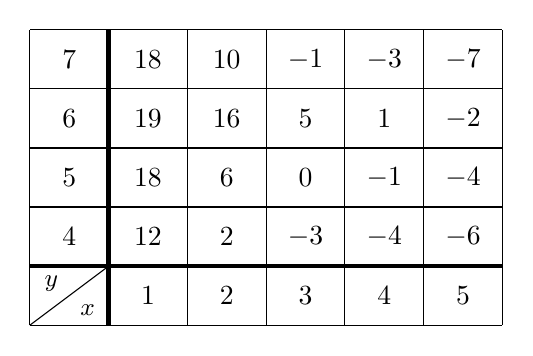
\begin{tikzpicture}[x=1cm,y=.75cm]
        \draw (0,0) grid [step=1] (6,5);
        
        \draw[ultra thick] (0,1)--(6,1);
        \draw[ultra thick] (1,0)--(1,5);
        
        \draw (0,0) -- (1,1);
        \node at (.4,.9) [below left,inner sep=1pt] {\small$y$};
        \node at (0.6,.1) [above right,inner sep=1pt] {\small$x$};
    
        %% y-values
        \node at (0.5,4.5) {$7$};
        \node at (0.5,3.5) {$6$};
        \node at (0.5,2.5) {$5$};
        \node at (0.5,1.5) {$4$};
        
        
        %% z-values
        %% top
        \node at (1.5,4.5) {$18$};
        \node at (2.5,4.5) {$10$};
        \node at (3.5,4.5) {$-1$};
        \node at (4.5,4.5) {$-3$};
        \node at (5.5,4.5) {$-7$};
        
        %% 
        \node at (1.5,3.5) {$19$};
        \node at (2.5,3.5) {$16$};
        \node at (3.5,3.5) {$5$};
        \node at (4.5,3.5) {$1$};
        \node at (5.5,3.5) {$-2$};
        
        %% 
        \node at (1.5,2.5) {$18$};
        \node at (2.5,2.5) {$6$};
        \node at (3.5,2.5) {$0$};
        \node at (4.5,2.5) {$-1$};
        \node at (5.5,2.5) {$-4$};
        
        %% 
        \node at (1.5,1.5) {$12$};
        \node at (2.5,1.5) {$2$};
        \node at (3.5,1.5) {$-3$};
        \node at (4.5,1.5) {$-4$};
        \node at (5.5,1.5) {$-6$};
        
        %% bottom row
        \node at (1.5,.5) {$1$};
        \node at (2.5,.5) {$2$};
        \node at (3.5,.5) {$3$};
        \node at (4.5,.5) {$4$};
        \node at (5.5,.5) {$5$};
      \end{tikzpicture}
    \end{image}
    Estimate the total differential $\d F$ in terms of $\d x$ and $\d
    y$ at the point $(2,6)$.
    \begin{explanation}
      We estimate $\grad F(2,6)$ as $\vector{\answer[given]{-7},\answer[given]{2}}$. Hence
      \[
      \d F \approx \answer[given]{-7}\d x + \answer[given]{2}\d y.
      \]
    \end{explanation}
\end{example}











\section{Approximating with the total differential}

Suppose you want to approximate $F(x,y)=\sqrt{x}\sin(y)$ at the point
$(4.1,0.8)$. \textbf{Without knowledge of calculus}, your approximation might
go like this:
\begin{quote}
  We try to find numbers near $4.1$ and $0.8$ where
  $F(x,y)=\sqrt{x}\sin(y)$ is easy to evaluate. For example, we know
  that $\sqrt{4}= 2$, so instead of looking at $x=4.1$, we'll use
  $x=4$. Also, we know $\sin(\pi/4)= \sqrt{2}/2$ since $\pi/4\approx
  0.8$, we'll use it in our approximation. Hence
  \begin{align*}
  F(4.1,0.8) &\approx F(4,\pi/4) \\
  &= \sqrt{4}\sin(\pi/4)\\
  &= 2\left(\frac{\sqrt{2}}2\right)\\
  &= \sqrt{2}.
  \end{align*}
\end{quote}
\textbf{Without calculus}, (or some other insight) this is the best
approximation we could reasonably come up with. The total differential
gives us a way of adjusting this initial approximation to hopefully
get a more accurate answer.

\begin{example}
  Let $F(x,y)=\sqrt{x}\sin(y)$. Approximate $F(4.1,0.8)$.
  \begin{explanation}
    By the definition, when $F$ is differentiable $\d F$ is a good
    approximation for $\Delta F$ when $\d x$ and $\d y$ are
    \wordChoice{\choice{large}\choice[correct]{small}}.

    As before we will attempt to compute $F(4.1,0.8)$ using
    $F(\answer[given]{4},\answer[given]{\pi/4})$. Recall from directly above
    \[
    F(4,\pi/4) = \answer[given]{\sqrt{2}}
    \]
    Now we will use the total differential to acquire a better
    approximation.  Consider
    \[
    \Delta F = F(4.1,0.8) - F(4,\pi/4).
    \]
    Since $\Delta F\approx \d F$, we write
    \begin{align*}
      \d F &\approx F(4.1,0.8) - F(4,\pi/4)\\
      F(4.1,0.8) &\approx F(4,\pi/4)+ \d F 
    \end{align*}
    To find $\d F$, we need $\grad F$, as
    \begin{align*}
      \d F &= \grad F \dotp \d\vec{x}\\
      &=\vector{\answer[given]{\frac{\sin (y)}{2\sqrt{x}}},\answer[given]{\sqrt{x}\cos (y)}}\dotp\vector{\d x,\d y}
    \end{align*}
    Evaluating at $(4,\pi/4)$ we find
    \begin{align*}
      \d F &= \grad F \dotp \d\vec{x}\\
      &=\vector{\answer[given]{\frac{\sin (\pi/4)}{2\sqrt{4}}}, \answer[given]{\sqrt{4}\cos (\pi/4)}}\dotp\vector{\d x,\d y }\\
      &=\vector{\frac{\sqrt{2}}{8}, \sqrt{2}}\dotp\vector{\d x,\d y }
    \end{align*}
    Now we need to know the change in $x$ and $y$:
    \begin{align*}
      \d x &= 4.1-4= \answer[given]{0.1}\\
    \d y &= 0.8 -\answer[given]{\pi/4} \approx 0.015.\\
    \end{align*}
    Thus
    \begin{align*}
      \d F &=  \vector{\answer[given]{\frac{\sqrt{2}}{8}}, \answer[given]{\sqrt{2}}}\dotp\vector{\answer[given]{0.1},\answer[given]{0.015}}\\ 
      &= \frac{\sqrt{2}}8(0.1) + \sqrt{2}(0.015)\\
    \end{align*}
    So finally,
    \begin{align*}
    F(4.1,0.8) &\approx F(4,\pi/4) + \d F\\
    F(4.1,0.8) &\approx \answer[given]{\sqrt{2} + \frac{\sqrt{2}}{8}(0.1) + \sqrt{2}(0.015)}
    \end{align*}
  \end{explanation}
\end{example}
\begin{remark}
  If we compare our estimates of $F(x,y) = \sqrt{x}\sin(y)$ at
  $(4.1,0.8)$ we see that without knowledge of calculus we found
  \[
  F(4.1,0.8) \approx \sqrt{2},
  \]
  but with knowledge of calculus we found
  \[
  F(4.1,0.8) \approx \sqrt{2} + \frac{\sqrt{2}}8(0.1) + \sqrt{2}(0.015)
  \]
  We can compute the actual value of $F(4.1,0.8)$ with a calculator.
  We find the value $1.45254$, accurate to $5$ places after the
  decimal. We see that calculus has served us well.
\end{remark}

The point of the previous example was \textit{not} to develop an
approximation method for known functions. After all, we can very
easily compute $F(4.1,0.8)$ using readily available
technology. Rather, it serves to illustrate how well this method of
approximation works, and to reinforce the following concept:
\begin{quote}
  New position = old position $+$ amount of change, \\
  New position $\approx$ old position + approximate amount of change.
\end{quote}

In the previous example, we could easily compute $F(4,\pi/4)$ and
could approximate the change in $F$ when computing $F(4.1,0.8)$,
letting us approximate the new value for $F$.

It may be surprising to learn that it is not uncommon to know the
values of $F$ and $\grad F$ at a particular point without actually
knowing a formula for $F$. The total differential gives a good method
of approximating $F$ by looking at nearby points.

\begin{example}
  Given that $F(2,-3) = 6$, $\grad F(2,-3) = \vector{1.3,-0.6}$,
  approximate $F(2.1,-3.03)$.
\begin{explanation}
  The total differential approximates how much $F$ changes from the
  point $(2,-3)$ to the point $(2.1,-3.03)$. With $\d x = \answer[given]{0.1}$ and $\d
  y = \answer[given]{-0.03}$, we have
  \begin{align*}
    \d F &= \grad F \dotp \d \vec{x}\\
    &= (1.3)(\answer[given]{0.1}) + (-0.6)(\answer[given]{-0.03}) \\
    &= 0.148.
  \end{align*}
  The change in $F$ is approximately $0.148$, so we approximate
  $F(2.1,-3.03)\approx \answer[given]{6.148}$.
\end{explanation}
\end{example}



\section{Error analysis}

The total differential gives an approximation of the change in $F$
given small changes in $x$ and $y$. We can use this to approximate
error propagation; that is, if the input is a little off from what it
should be, how far from correct will the output be? We demonstrate
this in an example.  \index{sensitivity analysis}\index{total
  differential!sensitivity analysis}

\begin{example}
  A cylindrical steel storage tank is to be built that is
  $10\unit{ft}$ tall and $4\unit{ft}$ across in diameter. It is known
  that the steel will expand/contract with temperature changes; is the
  overall volume of the tank more sensitive to changes in the diameter
  or in the height of the tank?
  \begin{explanation}
    A cylindrical solid with height $h$ and radius $r$ has volume
    \[
    V = \pi r^2h.
    \]
    We can view $V$ as a function of two variables, $r$ and $h$ (in
    that order). We can compute $\grad V$
    \[
    \grad V  = \vector{\answer[given]{2\pi r h},\answer[given]{\pi r^2}}.
    \]
    Setting $\vec{x}=\vector{r,h}$, the total differential is
    \begin{align*}
    \d V &=\grad V \dotp \d \vec{x}\\
    &=\vector{\answer[given]{2\pi rh},\answer[given]{ \pi r^2}}\dotp\vector{\d r,\d h}
    \end{align*}
    When $h = 10$ and $r = 2$, we have
    \[
    \d V = 40\pi \d r + 4\pi \d h.
    \]
    Note that the coefficient of $\d r$ is $40\pi\approx 125.7$; the
    coefficient of $\d h$ is \wordChoice{\choice[correct]{a tenth of
        that}\choice{ten times that}}, approximately $12.57$. A small
    change in radius will be multiplied by $125.7$, whereas a small
    change in height will be multiplied by $12.57$. Thus the volume of
    the tank is more sensitive to changes in radius than in height.
  \end{explanation}
\end{example}

The previous example showed that the volume of a particular tank was
more sensitive to changes in radius than in height. Keep in mind that
this analysis only applies to a tank of the dimensions given in the
problem. A tank with a height of $1$ft and radius of $5$ft would be
more sensitive to changes in height than in radius.

One could make a chart of small changes in radius and height and find
exact changes in volume given specific changes. While this provides
exact numbers, it does not give as much insight as the error analysis
using the total differential.

\end{document}
